\documentclass[10pt,a4paper,twoside]{article}

\usepackage{fullpage}
\usepackage[hidelinks]{hyperref}
\usepackage{booktabs}
\usepackage{graphicx}
\usepackage{setspace}
\onehalfspacing


\title{Installing iNZightVIT for Mac}
\author{\url{inzight_support@stat.auckland.ac.nz}}
\date{August 2014}

\begin{document}
\maketitle

The installation process for iNZight for Mac can be complicated, and is dependent on the
version of OS X. Therefore, the first thing you must to is check your version of Mac. Once
you have done this, follow the relevant installation instructions.

If you are unable to run iNZight after following the instructions, please check the
Troubleshooting section. If you still have problems, email
\href{mailto:inzight\_support@stat.auckland.ac.nz}{\url{inzight\_support@stat.auckland.ac.nz}}
(please include as much information as possible, including the version of mac you are
using, the steps you followed, etc.).

\section{Check your Mac OS X version}

\begin{itemize}
\item Click the ``Apple'' logo in the top-left corner of your screen

\item Click ``About this mac''

\item You will see the version of Mac you are using as \verb+Version 10.x.y+. (in the
  example below, the version is 10.7.4).
  \begin{center}
    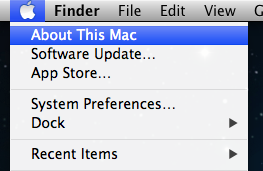
\includegraphics[width=0.4\textwidth]{fig/mac-aboutmymac1.png} \hspace{1em}
    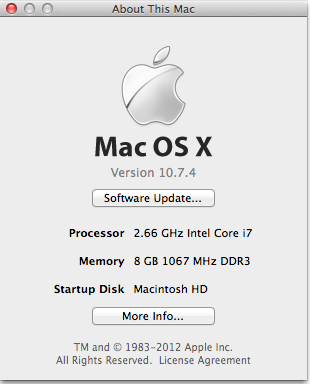
\includegraphics[width=0.4\textwidth,trim=0cm 6cm 0cm 1.5cm,clip=TRUE]{fig/mac-aboutmymac2.png}
  \end{center}

\end{itemize}

Now follow the relevant instructions for your version.

\vfill
\tableofcontents

\vfill\pagebreak
\section{Install iNZight}
\subsection{Mavericks - OS X 10.9}
\label{inst-mav}

\textbf{NOTE:} \emph{This is the most recent release of Mac OS X. If you have the most
  recent release, there may be compatibility issues running iNZight and the required
  software. Please let us know if iNZight stops working for you after an OS X update.}


\begin{enumerate}
\item \textbf{Download the necessary software}
  \begin{itemize}
  \item \textbf{XQuartz - download and run the installation wizard}

    The most recent version can be found at:\\ \url{http://xquartz.macosforge.org/landing/}

    If you have troubles with this version, try an older version from here:\\
    \url{http://xquartz.macosforge.org/trac/wiki/Releases} (your best chance is with X11
    2.7.5)

  \item \textbf{GTK+ - download and run the installation wizard}

    This can be downloaded directly from\\ \url{http://r.research.att.com/libs/GTK_2.24.17-X11.pkg}

  \item \textbf{iNZightVIT for Mavericks - download and unzip}
    
    Download the \verb+zip+ file from the website:\\
    \url{https://www.stat.auckland.ac.nz/~wild/iNZight/mac.html#mavericks}

    (If it doesn't do it automatically, unzip the folder.)
  \end{itemize}

\item \textbf{Restart your computer} - this is important for the installation of GTK.

\item \textbf{Allow iNZight access} - the default security settings on Mavericks wont
  allow iNZight to run

  \begin{itemize}
  \item Open the \verb+iNZightVIT_2.x.y+ folder
  \item Right-click \verb+R.app+ and select \verb+Open+
  \item In the window that pops up, click \verb+Open+
  \end{itemize}

\item \textbf{Update iNZight} - this step is usually not required, but to ensure
  everything is as up-to-date as possible:
  \begin{itemize}
  \item Open the \verb+iNZightVIT_2.x.y+ folder you have unzipped
  \item \emph{For the first time running the update:}

    -- Right-click \verb+UPDATE_iNZightVIT.command+ and select \verb+Open+\\
    -- Click \verb+Open+ in the window the pops up.
    
    In future, you can simply double-click to open.

  \item You may need to run the program several times to finish all updates. You will know
    it's finished when you see the following message:
  \end{itemize}

\item \textbf{Run iNZight}

  \begin{itemize}
  \item \emph{For the first time running iNZight:}

    -- Right-click \verb+START_iNZightVIT.command+ and select \verb+Open+\\
    -- Click \verb+Open+ in the window the pops up.

    In future, you can simply double-click \verb+START_iNZight.command+

  \item If you experience performance issues (iNZight lagging, running slowly) then ``App
    nap'' might be the culprit.
    
    -- Right-click \verb+START_iNZightVIT.command+ and select ``Get info''\\
    -- In the window that opens, check the box next to ``Prevent app nap''
  \end{itemize}

\end{enumerate}




\vfill\pagebreak
\subsection{Mountain Lion - OS X 10.8}

\begin{enumerate}
\item \textbf{Download the necessary software}
  \begin{itemize}
  \item \textbf{XQuartz - download and run the installation wizard}

    Download the necessary version from\\
    \url{http://xquartz.macosforge.org/trac/wiki/X112.7.5}

    Double click the downloaded file and you should see \verb+XQuartz-2.7.5+ appear on
    your desktop. Double click this to get the following window:
    \begin{center}
      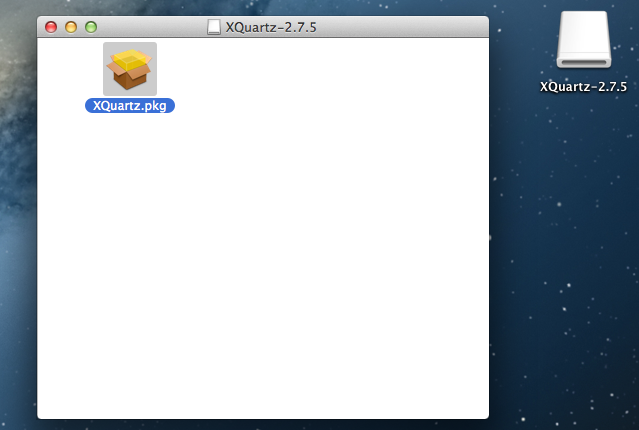
\includegraphics[width=0.5\textwidth,trim=0cm 5cm 0cm 0cm,clip=TRUE]{fig/mountain-lion/s1-c.png}
    \end{center}

    Double click \verb+XQuartz.pkg+ to launch the installer for XQuartz.
    \begin{center}
      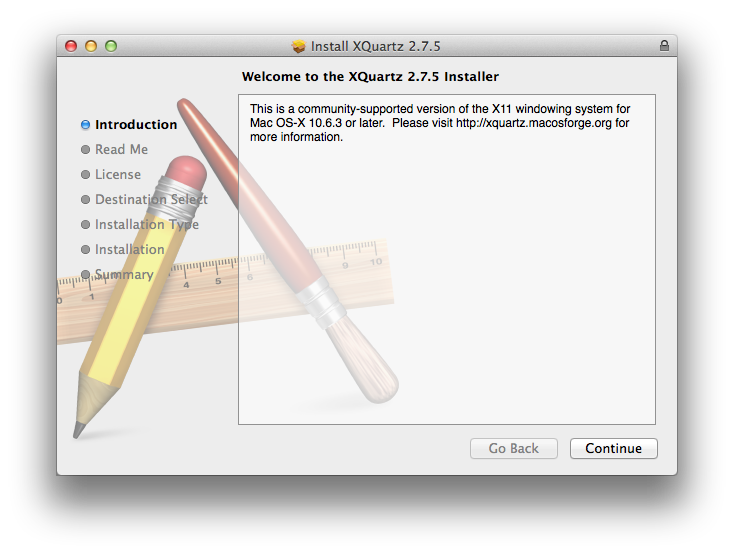
\includegraphics[width=0.5\textwidth]{fig/mountain-lion/s1-d.png}
    \end{center}
    
    If installation is OK, you should see the following screen:
    \begin{center}
      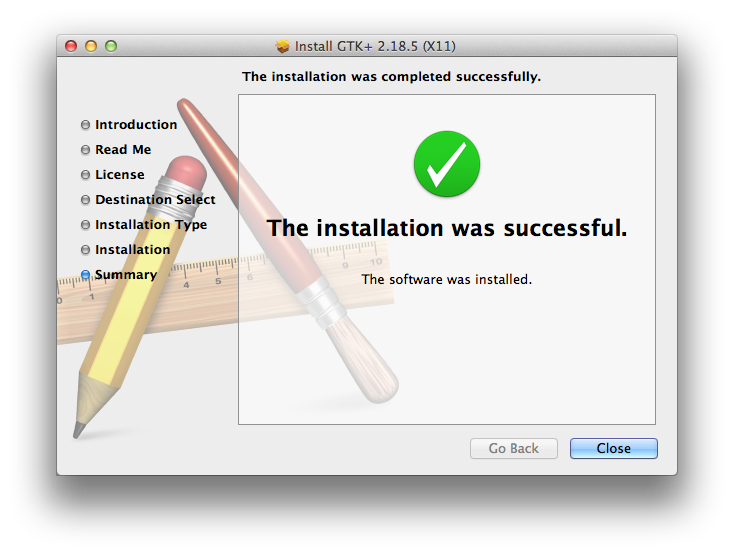
\includegraphics[width=0.5\textwidth]{fig/mountain-lion/s1-b.png}
    \end{center}
    
    The software may ask you to update XQuartz. This is not required for iNZight, and is
    not recommended as it may cause issues. If you accidentally udpate, simply redownload
    and install the above version.

   

  \item \textbf{GTK+ - download and run the installation wizard}

    This can be downloaded directly from\\ 
    \url{http://r.research.att.com/libs/GTK_2.18.5-X11.pkg}
    
    Double click the \verb+GTK_2.18.5-X11.pkg+ file you downloaded to launch the installer:
    \begin{center}
      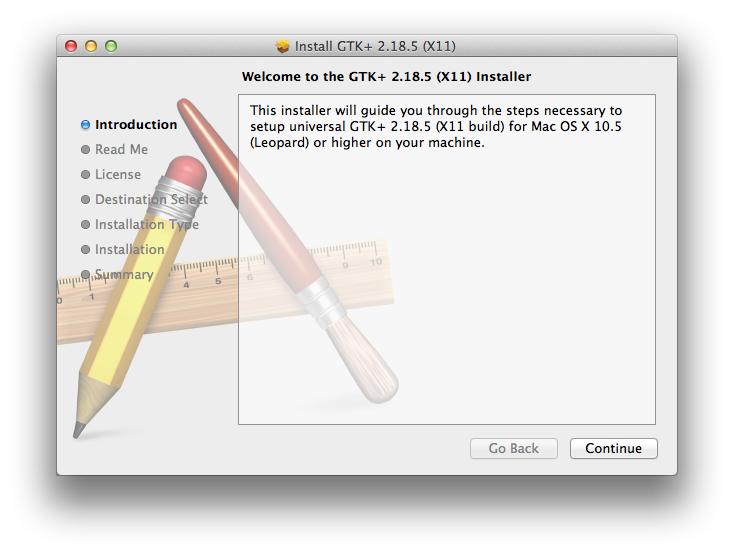
\includegraphics[width=0.5\textwidth]{fig/mountain-lion/s1-a.png}
    \end{center}
    
    If installation is OK, you should see the following screen:
    \begin{center}
      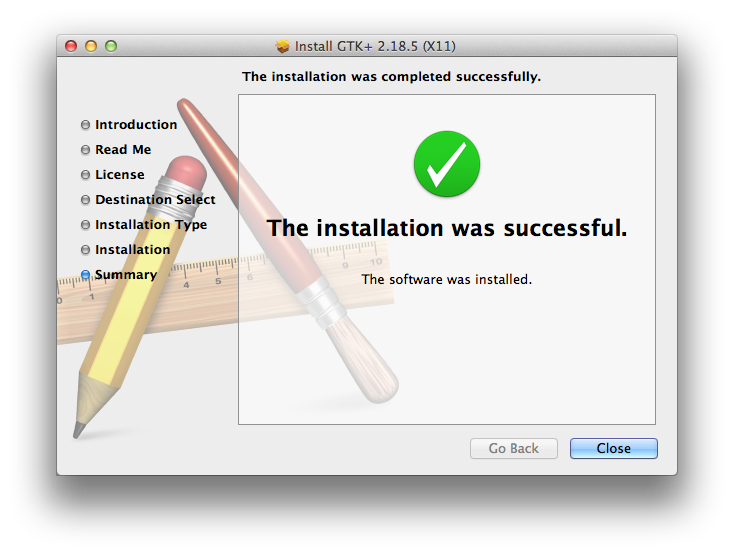
\includegraphics[width=0.5\textwidth]{fig/mountain-lion/s1-b.png}
    \end{center}

  \item \textbf{iNZightVIT for Previous Mac Versions - download and unzip}
    
    Download the \verb+zip+ file from the website:\\
    \url{https://www.stat.auckland.ac.nz/~wild/iNZight/mac.html#snowleopard}

    

    (If it doesn't do it automatically, unzip the folder.)
  \end{itemize}

\item \textbf{Restart your computer} - this is important for the installation of GTK.

\vfill
{\flushright continued on next page \ldots}
\pagebreak
\item \textbf{Allow iNZight access} - the default security settings on Mountain Lion wont
  allow iNZight to run

  \begin{itemize}
  \item Open the \verb+iNZightVIT_2.x.y-snowleopard+ folder
  \item Right-click \verb+R64+ and select \verb+Open+
  \item In the window that pops up, click \verb+Open+
    \begin{center}
      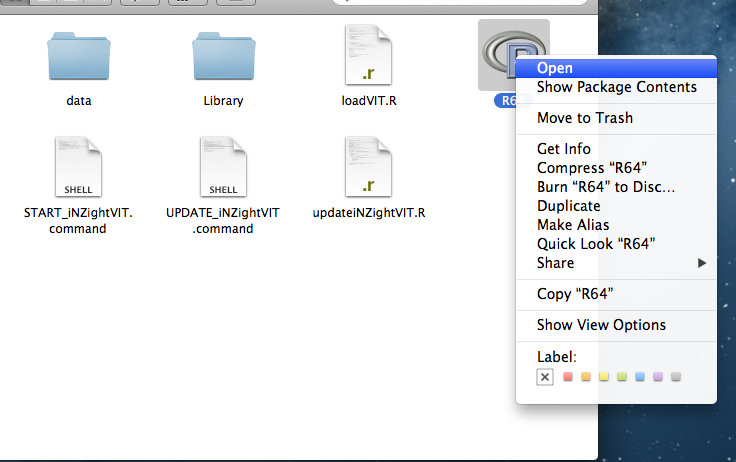
\includegraphics[width=0.4\textwidth]{fig/mountain-lion/s2-a.png}
      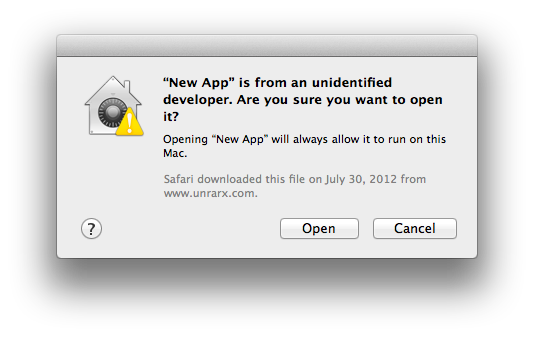
\includegraphics[width=0.4\textwidth]{fig/open-unknown.png}  %% make unique one ?
    \end{center}
  \end{itemize}

\item \textbf{Run iNZight}

  \begin{itemize}
  \item \emph{For the first time running iNZight:}

    -- Right-click \verb+START_iNZightVIT.command+ and select \verb+Open+\\
    -- Click \verb+Open+ in the window the pops up.
    \begin{center}
      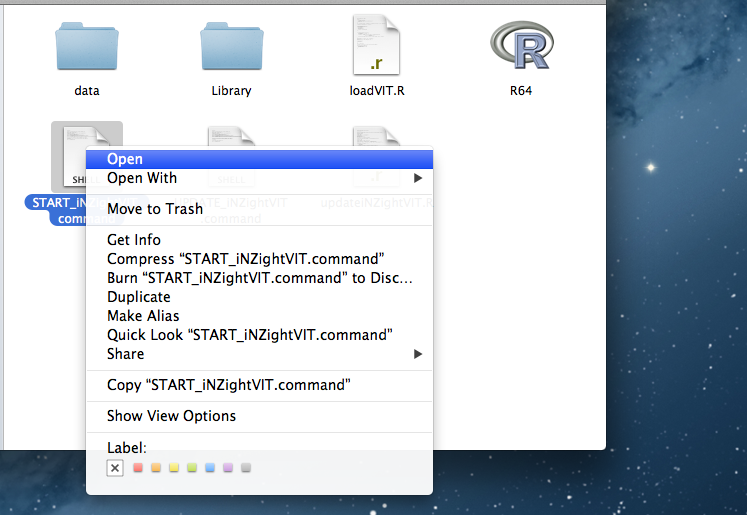
\includegraphics[width=0.4\textwidth]{fig/mountain-lion/s2-b.png}
      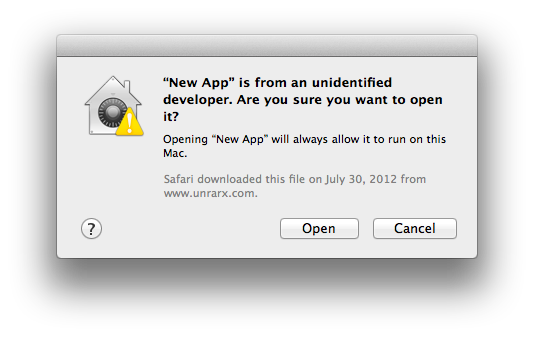
\includegraphics[width=0.4\textwidth]{fig/open-unknown.png}  %% make unique one ?
    \end{center}

    In future, you can simply double-click to launch iNZight.

  \end{itemize}

\item \textbf{Optional - Update iNZight}
  You may want to periodically update your copy of iNZight.

  \begin{itemize}
  \item \emph{For the first time running the update:}

    -- Right-click \verb+UPDATE_iNZightVIT.command+ and select \verb+Open+\\
    -- Click \verb+Open+ in the window the pops up.
    
    In future, you can simply double-click to update.

  \item You may need to run the program several times to finish all updates. You will know
    it's finished when you see the following message:
  \end{itemize}
 
\end{enumerate}


\vfill\pagebreak
\subsection{Lion and Snow Leopard - OS X 10.7 and 10.6}

\begin{enumerate}
\item \textbf{Download the necessary software}
  \begin{itemize}

  \item \textbf{GTK+ - download and run the installation wizard}

    This can be downloaded directly from\\ 
    \url{http://r.research.att.com/libs/GTK_2.18.5-X11.pkg}

    Double click the \verb+GTK_2.18.5-X11.pkg+ file you downloaded to launch the installer:
    \begin{center}
      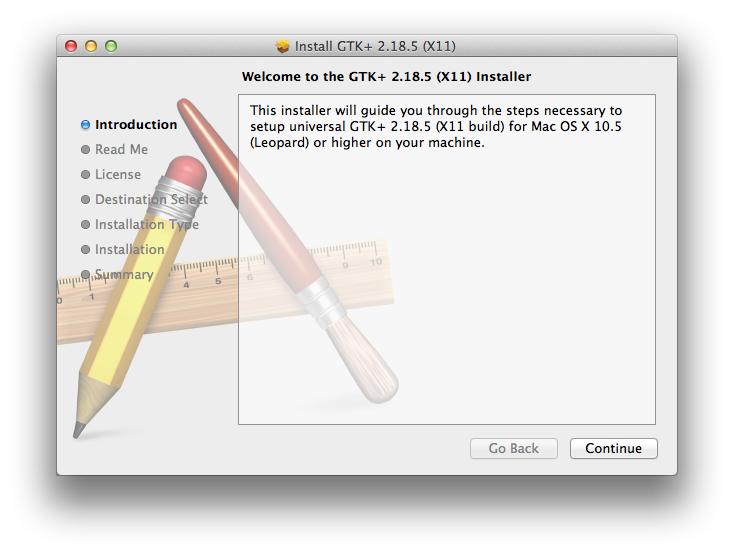
\includegraphics[width=0.5\textwidth]{fig/mountain-lion/s1-a.png}
    \end{center}
    
    If installation is OK, you should see the following screen:
    \begin{center}
      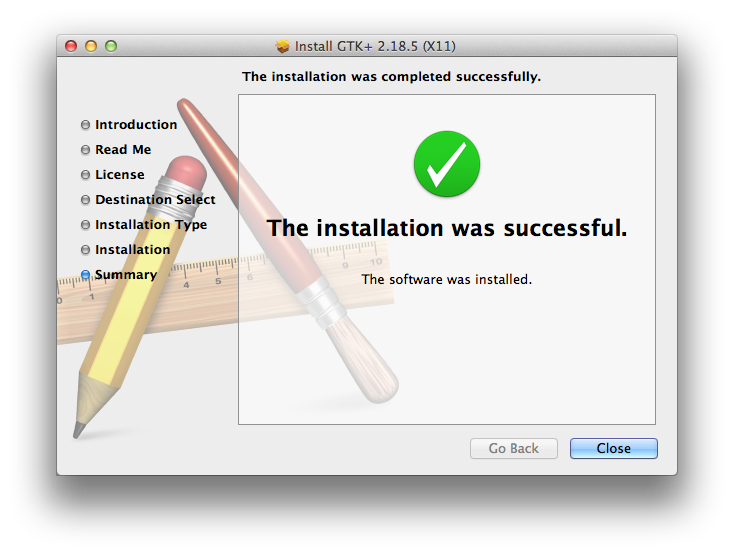
\includegraphics[width=0.5\textwidth]{fig/mountain-lion/s1-b.png}
    \end{center}

  \item \textbf{iNZightVIT for Previous Mac Versions - download and unzip}
    
    Download the \verb+zip+ file from the website:\\
    \url{https://www.stat.auckland.ac.nz/~wild/iNZight/mac.html#snowleopard}

    (If it doesn't do it automatically, unzip the folder.)
  \end{itemize}

\item \textbf{Restart your computer} - this is important for the installation of GTK.

\item \textbf{Run iNZight} - Double-click \verb+START_iNZight.command+


\item \textbf{Optional - Update iNZight}
  You may want to periodically update your copy of iNZight.

  \begin{itemize}
  \item Double-click to open.

  \item You may need to run the program several times to finish all updates. You will know
    it's finished when you see the following message:
  \end{itemize}
 
\end{enumerate}



\vfill\pagebreak
\section{Troubleshooting}
\setlength{\parindent}{0pt}

\textbf{When I run iNZight, the ``Loading iNZight'' window opens, but then nothing happens.}

This usually happens if iNZight cannot find XQuartz. Make sure you have downloaded the
most recent version of XQuartz and run the update iNZight program.


\vspace{1em}
\textbf{I see the error message ``R session is headerless'' when I try running iNZight.}

Make sure you have restarted your mac after installing GTK. If you continue to get the
error message, try reinstalling GTK, restart, and try again.


\vspace{1em}
\textbf{iNZight lags or runs really slowly on Mavericks.}

Make sure you have disabled ``App nap''. Right-click the \verb+START_iNZightVIT.command+
icon and select ``Get info''. Check the box next to ``Prevent app nap''. See step 5.\ of
section \ref{inst-mav} for more detailed instructions.

\begin{center}
  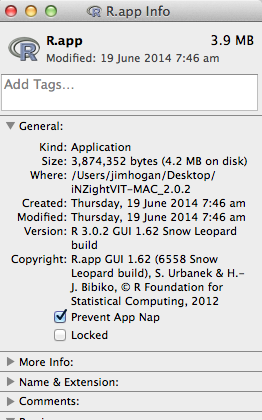
\includegraphics[width=0.4\textwidth]{fig/mavericks/preventappnap.png}
\end{center}


\vspace{1em}
\textbf{How do I save my graphs from the VIT module?}

You can do this by creating a screen shot of the window.
\begin{itemize}
\item Press Command + Shift + 4 on your keyboard
\item Either:
  \begin{itemize}
  \item[A:] Click and drag to select the figure to save, or
  \item[B:] press the Space Bar and then click the window you want to save
  \end{itemize}
\item Your selected image will be saved to the desktop
\end{itemize}


\vspace{1em}
\textbf{I'm still stuck, and don't know what to do!}

If you can, go here: \url{https://www.stat.auckland.ac.nz/~wild/iNZight/report.php} and
fill in the form with as much detail as you can.

If you can't access the page, please send an email to
\href{mailto:inzight\_support@stat.auckland.ac.nz}{inzight\_support@stat.auckland.ac.nz}
and we will get back to you ASAP. Please include as much information as possible,
including:
\begin{itemize}
\item You mac version
\item What part of iNZight you are using (the VIT of iNZight module)
\item What you did to get stuck --- if you have strange messages on your screen, take a
  screen shot (Command + Shift + 3) and attach it to the email
\item Any other information that might help solve the problem
\end{itemize}


\end{document}
